\section{Brugsscenarier}
\label{TestAfSkalaBrugsscenarier}
%
Brugsscenarierne til evalueringen med skalaerne svarer til dem, der blev anvendt i feltundersøgelsen, som er præsenteret i \autoref{ParametreBrugsscenarier}. Ved brugsscenariet hvor der vælges destination, er antallet af afgange dog ændret fra fire til fem, for at tilpasse destinationerne efter de reelle afgange der er på den pågældende dag, hvor evalueringen udføres. De fem destinationer de rejsende kan vælge imellem fremgår af højre side på \autoref{fig:TilpassetDestination}, hvor venstre side gengiver skærmbilledet fra feltundersøgelsen. 
%
\begin{figure}[H]
\centering
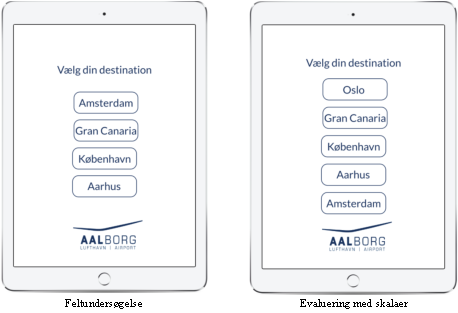
\includegraphics[width =0.8\textwidth]{Figure/TestdesignEvaluering/TilpassetDestination} 
\caption{Illustration af ændringerne foretaget fra feltundersøgelsen (venstre) til evalueringen med skalaerne (venstre).}
\label{fig:TilpassetDestination}
\end{figure}
\noindent
%
Udover ændringen i hvilke destinationer der kan vælges, er informationen til den specifikke destination ligeledes tilpasset så det svarer til informationerne fundet på Aalborg Lufthavns hjemmeside for den 01/12-2017. 